\section{离散LTI系统的卷积模型}

本节介绍离散LTI系统在时域的卷积模型。

本节要点:
\begin{itemize}
    \item 了解卷积和的概念;
    \item 熟悉卷积和的物理意义;
    \item 熟悉Numpy的卷积函数。
\end{itemize}

%============================================================
\subsection{卷积的导出过程}

\begin{definition}[冲激响应]
我们称单位冲激信号$\delta \left[ n \right] $经过零状态系统后的输出为{\bf 单位冲激响应},简称{\bf 冲激响应}(pulse response),记为$h\left[ n \right] $。
\end{definition}

继续以RC电路为例,取采样间隔0.2s,差分方程:
\[
y\left[ n \right] =0.8y\left[ n-1 \right] +0.2x\left[ n-1 \right] \qquad n=0,1,2,\cdots
\]
对于冲激输入,我们可以通过之前的方法获得其响应,如下左图。
由于系统的LTI性,对于等比例冲激输入和时移的冲激输入,都有同样的等比输出和时移输出。
假设时移并放大至$3\delta \left[ n-4 \right] $,响应如下右图。
\begin{figure}[h]
\centering
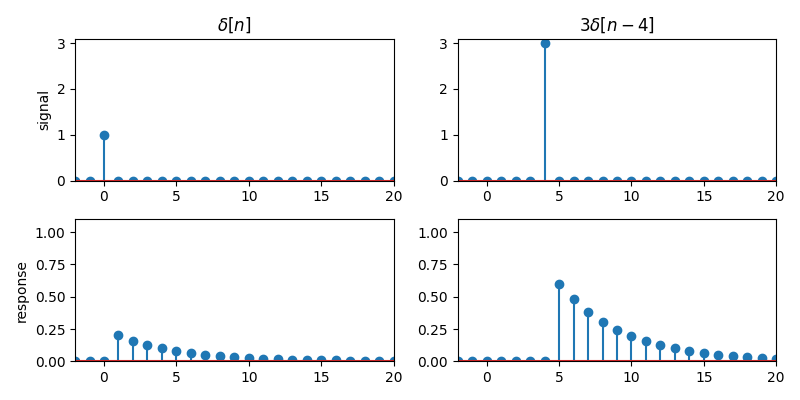
\includegraphics[height=5cm]{3.1.1-1.png}
\end{figure}

由于输入信号可以视为一系列冲激的和,相应地,输出信号也可以视为一系列冲激响应的和:
\begin{align*}
&x\left[ n \right] =\sum_{i=0}^{\infty}{x\left[ i \right] \delta \left[ n-i \right]} \qquad n=0,1,2,\cdots \\
&y\left[ n \right] =\sum_{i=0}^{\infty}{x\left[ i \right] h\left[ n-i \right]} \qquad n=0,1,2,\cdots
\end{align*}

举例说明,假设输入信号$x\left[ n \right] $和系统的冲激响应$h\left[ n \right] $如下:
\begin{figure}[ht]
\centering
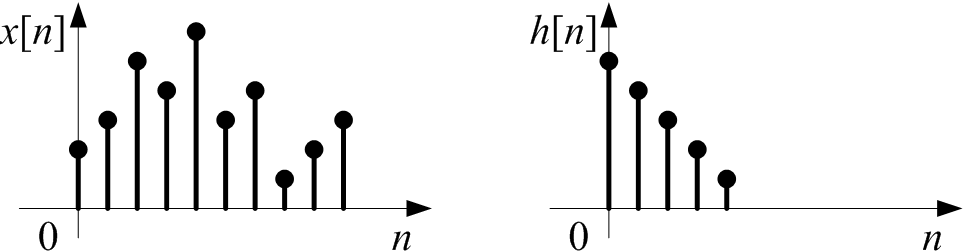
\includegraphics[height=2cm]{3.1.1-3.png}
\end{figure}

若要获得输出$y\left[ 3 \right] $,则系统会对输入$x\left[ 0 \right] ,x\left[ 1 \right] ,x\left[ 2 \right] ,x\left[ 3 \right] $进行“加权叠加响应”,如下左图。
如果要获得输出$y\left[ 9 \right] $,由于系统的响应只到$h\left[ 4 \right] $,所以系统只对$x\left[ 5 \right] ,x\left[ 6 \right] ,x\left[ 7 \right] ,x\left[ 8 \right] ,x\left[ 9 \right] $进行“加权叠加响应”,如下右图。
\begin{figure}[h]
\centering
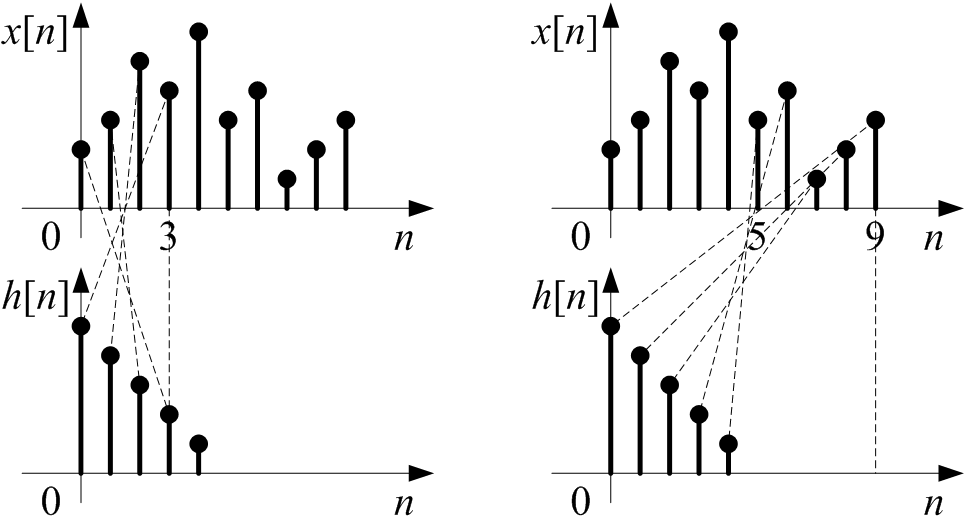
\includegraphics[height=4cm]{3.1.1-4.png}
\end{figure}

从数学角度看,$n$刻的输出$y\left[ n \right] $是$n$刻及之前时刻的输入$x\left[ i \right] ,i=0,1,2,\cdots ,n$的加权和,对应的权重为$h\left[ n-i \right] ,i=0,1,2,\cdots ,n$,可以理解“翻转+时移”。
\begin{figure}[h]
\centering
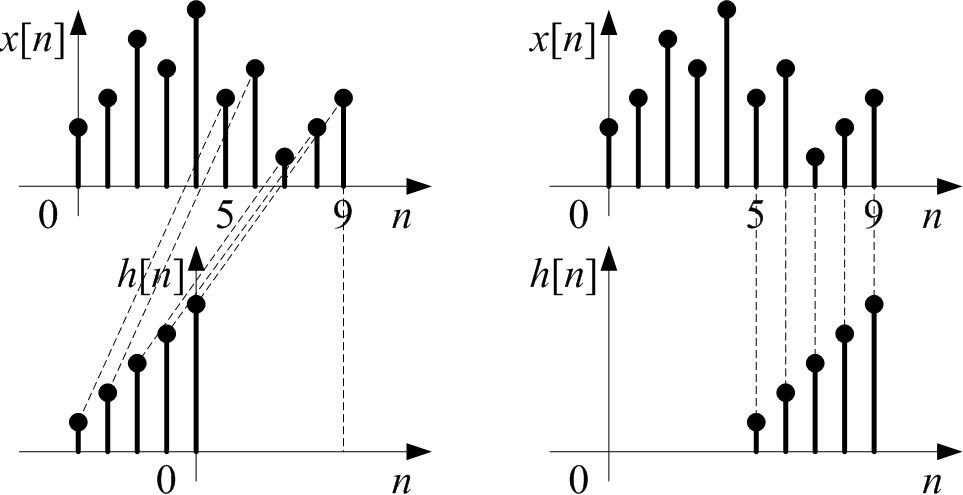
\includegraphics[height=4cm]{3.1.1-5.png}
\end{figure}
\[
y\left[ n \right] =\left[ \begin{matrix}
	x\left[ 0 \right]&		x\left[ 1 \right]&		\cdots&		x\left[ n-1 \right]&		x\left[ n \right]\\
\end{matrix} \right] \cdot \left[ \begin{array}{c}
	h\left[ n \right]\\
	h\left[ n-1 \right]\\
	\vdots\\
	h\left[ 1 \right]\\
	n\left[ 0 \right]\\
\end{array} \right]
\]

%============================================================
\subsection{卷积和和卷积模型}

\begin{definition}[卷积和]
对于两个离散函数$a\left[ n \right] ,b\left[ n \right] ,n\in \mathbb{Z} $,如果和式$\sum_{i=-\infty}^{+\infty}{a\left[ i \right] b\left[ n-i \right]}$收敛,则称其为{\bf $a\left[ n \right] ,b\left[ n \right] $的卷积和}(convolution sum),记为$a\left[ n \right] \ast b\left[ n \right] $,即:
\[
a\left[ n \right] \ast b\left[ n \right] =\sum_{i=-\infty}^{+\infty}{a\left[ i \right] b\left[ n-i \right]}
\]
\end{definition}

可见,卷积和是“一个和,一个加权和,一个反置移位的加权和”。

~

{\bf 离散LTI系统的卷积模型}:设一离散LTI系统符合因果律且零状态,若对单位冲激信号$\delta \left[ n \right] $的响应$h\left[ n \right] $已知,则该系统对任何输入信号的响应可以表示为输入信号$x\left[ n \right] $和冲激响应$h\left[ n \right] $的卷积,即:
\[
y\left[ n \right] =x\left[ n \right] \ast h\left[ n \right] =\begin{cases}
	0 &n=-1,-2,\cdots\\
	\sum_{i=0}^n{x\left[ i \right] h\left[ n-i \right]} &n=0,1,2,\cdots\\
\end{cases}
\]
该表达式称为{\bf 系统的卷积模型}。

从混响和回响的角度,输出$y\left[ n \right] $可以理解为一系列输入产生的系统回响$x\left[ i \right] h\left[ n-i \right] $的叠加。
只是要特别注意,$i$刻的回响不是$x\left[ i \right] h\left[ i \right] $,而是$x\left[ i \right] h\left[ n-i \right] $。
如0刻的回响是$x\left[ 0 \right] h\left[ n \right] $,因为此时回响已经经历了时间$n$,$n$刻的回响是$x\left[ n \right] h\left[ 0 \right] $。

%============================================================
\subsection{差分方程模型和卷积模型}

至此,对于一个LTI系统,我们可以用差分方程和卷积两种方法描述:
\begin{align*}
&y\left[ n \right] +\sum_{i=1}^N{A_iy\left[ n-i \right]}=\sum_{i=0}^M{B_ix\left[ n-i \right]} \\
&y\left[ n \right] =x\left[ n \right] \ast h\left[ n \right]
\end{align*}
两种模型都要求系统是LTI,区别在于:
\begin{itemize}
    \item 差分方程要求是有限维度,用系数$A_1\cdots A_N,B_0,B_1,\cdots ,B_M$描述系统,不同系统的区别就在于不同的系数。
    \item 卷积要求符合因果律,用冲激响应$h\left[ n \right] $描述系统,不同系统的区别在于不同的$h\left[ n \right] $。
\end{itemize}

%============================================================
\subsection{卷积的物理意义}

结合记忆和因果,卷积的物理意义就很明显。
由于系统的内部构造,系统对输入的能量会有惯性,冲激能量$\delta \left[ n \right] $在内部会造成一个回响$h\left[ n \right] $。
只要系统是LTI,输出$y \left[ t \right]$就是此刻及之前每刻的回响的混响$\sum_{i=0}^n{x\left[ i \right] h\left[ n-i \right]}$。
回响是惯性的表现,混响是LTI的结果,所以卷积是LTI的必然结果。
若将系统分为几个子系统,由于LTI的关系,系统的最终表现与子系统在空间上的组合和时间上的前后无关,数学上表示为卷积的分配率和结合律。

%============================================================
\subsection{Python应用——numpy.convolve()函数}

numpy提供了卷积函数convolve()。
\begin{figure}[h]
\centering
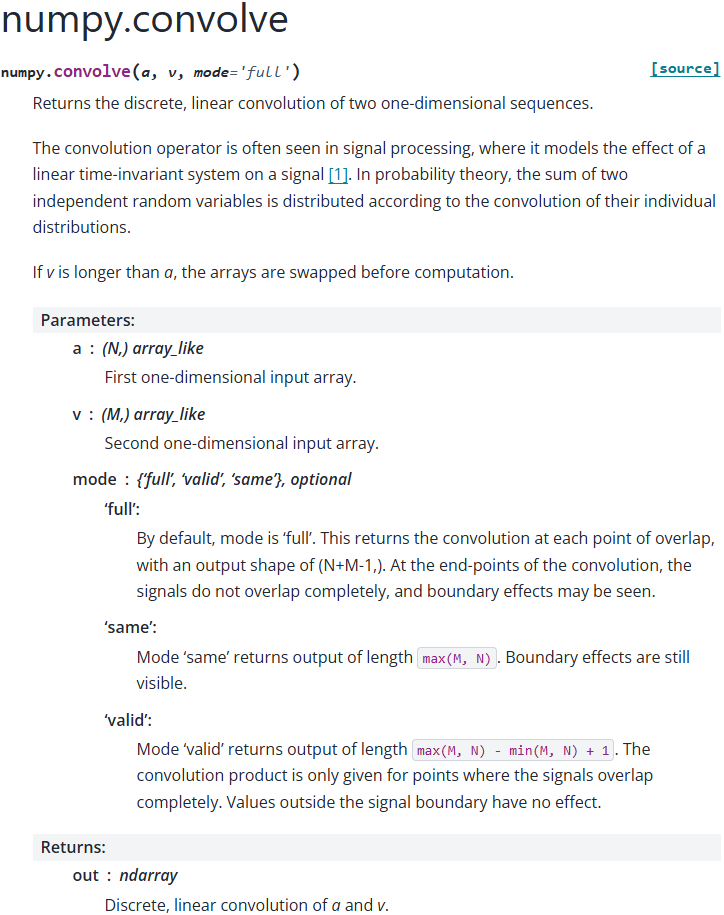
\includegraphics[width=10cm]{3.1.5-1.png}
\end{figure}

假设系统的差分方程为:
\[
y\left[ n \right] -0.8y\left[ n-1 \right] =0.2x\left[ n-1 \right]
\]
通过my\_diff函数可以获得冲激响应,取前11个值:
\begin{center}
h = [0, 0.2, 0.16, 0.128, 0.1024, 0.0819, 0.0655, 0.0524, 0.0419, 0.0336, 0.0268]
\end{center}
用np.convolve()计算冲激响应和输入信号(单位阶跃)的卷积,对比差分方程的计算:

\begin{python}
An = np.array([-0.8]); Bm = np.array([0.2]); b = 0
Yn = np.array([0]);    Xm = np.array([0])

n  = np.arange(-2, 21, 1)
X  = np.zeros_like(n, dtype=np.float64)
X[2:] = 1.0
Yd = my_diff(An, Yn, Bm, Xm, b, X)
h  = np.array([0.0, 0.2, 0.16, 0.128, 0.1024, 0.0819, 0.0655, 0.0524, 0.0419, 0.0336, 0.0268])
Yc = np.convolve(X, h, mode='full')
\end{python}

\begin{itemize}
    \item Yd是我们my\_diff()函数的计算结果;
    \item Yc是用Numpy的convolve()函数的计算结果,注意它认为输入是方波,所以长度会比较长,绘制Yc时需要截断;
    \item 由于我们的h只取了前11个,所以计算得到的值并没有“长足”。
\end{itemize}

\begin{figure}[h]
\centering
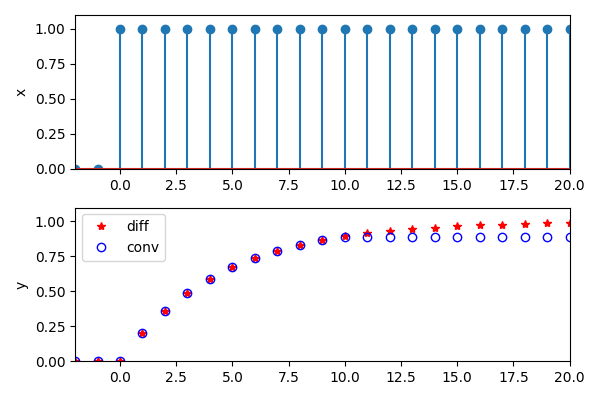
\includegraphics[height=5cm]{3.1.5-2.png}
\end{figure}




